\documentclass[twoside]{book}

% Packages required by doxygen
\usepackage{fixltx2e}
\usepackage{calc}
\usepackage{doxygen}
\usepackage{graphicx}
\usepackage[utf8]{inputenc}
\usepackage{makeidx}
\usepackage{multicol}
\usepackage{multirow}
\PassOptionsToPackage{warn}{textcomp}
\usepackage{textcomp}
\usepackage[nointegrals]{wasysym}
\usepackage[table]{xcolor}

% Font selection
\usepackage[T1]{fontenc}
\usepackage{mathptmx}
\usepackage[scaled=.90]{helvet}
\usepackage{courier}
\usepackage{amssymb}
\usepackage{sectsty}
\renewcommand{\familydefault}{\sfdefault}
\allsectionsfont{%
  \fontseries{bc}\selectfont%
  \color{darkgray}%
}
\renewcommand{\DoxyLabelFont}{%
  \fontseries{bc}\selectfont%
  \color{darkgray}%
}
\newcommand{\+}{\discretionary{\mbox{\scriptsize$\hookleftarrow$}}{}{}}

% Page & text layout
\usepackage{geometry}
\geometry{%
  a4paper,%
  top=2.5cm,%
  bottom=2.5cm,%
  left=2.5cm,%
  right=2.5cm%
}
\tolerance=750
\hfuzz=15pt
\hbadness=750
\setlength{\emergencystretch}{15pt}
\setlength{\parindent}{0cm}
\setlength{\parskip}{0.2cm}
\makeatletter
\renewcommand{\paragraph}{%
  \@startsection{paragraph}{4}{0ex}{-1.0ex}{1.0ex}{%
    \normalfont\normalsize\bfseries\SS@parafont%
  }%
}
\renewcommand{\subparagraph}{%
  \@startsection{subparagraph}{5}{0ex}{-1.0ex}{1.0ex}{%
    \normalfont\normalsize\bfseries\SS@subparafont%
  }%
}
\makeatother

% Headers & footers
\usepackage{fancyhdr}
\pagestyle{fancyplain}
\fancyhead[LE]{\fancyplain{}{\bfseries\thepage}}
\fancyhead[CE]{\fancyplain{}{}}
\fancyhead[RE]{\fancyplain{}{\bfseries\leftmark}}
\fancyhead[LO]{\fancyplain{}{\bfseries\rightmark}}
\fancyhead[CO]{\fancyplain{}{}}
\fancyhead[RO]{\fancyplain{}{\bfseries\thepage}}
\fancyfoot[LE]{\fancyplain{}{}}
\fancyfoot[CE]{\fancyplain{}{}}
\fancyfoot[RE]{\fancyplain{}{\bfseries\scriptsize Generated on Fri May 8 2015 23\+:40\+:22 for Pong Game by Doxygen }}
\fancyfoot[LO]{\fancyplain{}{\bfseries\scriptsize Generated on Fri May 8 2015 23\+:40\+:22 for Pong Game by Doxygen }}
\fancyfoot[CO]{\fancyplain{}{}}
\fancyfoot[RO]{\fancyplain{}{}}
\renewcommand{\footrulewidth}{0.4pt}
\renewcommand{\chaptermark}[1]{%
  \markboth{#1}{}%
}
\renewcommand{\sectionmark}[1]{%
  \markright{\thesection\ #1}%
}

% Indices & bibliography
\usepackage{natbib}
\usepackage[titles]{tocloft}
\setcounter{tocdepth}{3}
\setcounter{secnumdepth}{5}
\makeindex

% Hyperlinks (required, but should be loaded last)
\usepackage{ifpdf}
\ifpdf
  \usepackage[pdftex,pagebackref=true]{hyperref}
\else
  \usepackage[ps2pdf,pagebackref=true]{hyperref}
\fi
\hypersetup{%
  colorlinks=true,%
  linkcolor=blue,%
  citecolor=blue,%
  unicode%
}

% Custom commands
\newcommand{\clearemptydoublepage}{%
  \newpage{\pagestyle{empty}\cleardoublepage}%
}


%===== C O N T E N T S =====

\begin{document}

% Titlepage & ToC
\hypersetup{pageanchor=false,
             bookmarks=true,
             bookmarksnumbered=true,
             pdfencoding=unicode
            }
\pagenumbering{roman}
\begin{titlepage}
\vspace*{7cm}
\begin{center}%
{\Large Pong Game }\\
\vspace*{1cm}
{\large Generated by Doxygen 1.8.8}\\
\vspace*{0.5cm}
{\small Fri May 8 2015 23:40:22}\\
\end{center}
\end{titlepage}
\clearemptydoublepage
\tableofcontents
\clearemptydoublepage
\pagenumbering{arabic}
\hypersetup{pageanchor=true}

%--- Begin generated contents ---
\chapter{Pong\+Game Instruction}
\label{index}\hypertarget{index}{}\hypertarget{index_intro_sec}{}\section{Introduction}\label{index_intro_sec}
Welcome to the introduction of Pong Game!

This is a Pong Game designed by Zixiao Wang.

This introduction will introduce the basic control of the game.\hypertarget{index_intro_sec}{}\section{Introduction}\label{index_intro_sec}
There will be a control panel besides the game window help you to control the game. It is easy to learn how to play the game. Choose one of Modes showed on the panel, game will start automaticlly. R\+E\+M\+E\+M\+B\+E\+R to click the window after you choose the game mode, otherwise you will could not control the paddle!!

Left Mouse Click\+: start/pause

\hyperlink{classPlayer}{Player} 1 (Top paddle)\+:~\newline
a -\/$>$ move left ~\newline
d -\/$>$ move right

\hyperlink{classPlayer}{Player} 2 (Bottom paddle) \+: ~\newline
left key -\/$>$ move left~\newline
right key -\/$>$ move right 
\chapter{Hierarchical Index}
\section{Class Hierarchy}
This inheritance list is sorted roughly, but not completely, alphabetically\+:\begin{DoxyCompactList}
\item \contentsline{section}{Ball}{\pageref{classBall}}{}
\item \contentsline{section}{Base\+Gfx\+App}{\pageref{classBaseGfxApp}}{}
\begin{DoxyCompactList}
\item \contentsline{section}{Simulation}{\pageref{classSimulation}}{}
\end{DoxyCompactList}
\item \contentsline{section}{Player}{\pageref{classPlayer}}{}
\item \contentsline{section}{Pong\+Game}{\pageref{classPongGame}}{}
\end{DoxyCompactList}

\chapter{Class Index}
\section{Class List}
Here are the classes, structs, unions and interfaces with brief descriptions\+:\begin{DoxyCompactList}
\item\contentsline{section}{\hyperlink{classBall}{Ball} \\*\hyperlink{classBall}{Ball} class represents the ball in game }{\pageref{classBall}}{}
\item\contentsline{section}{\hyperlink{classBaseGfxApp}{Base\+Gfx\+App} }{\pageref{classBaseGfxApp}}{}
\item\contentsline{section}{\hyperlink{classPlayer}{Player} \\*The \hyperlink{classPlayer}{Player} class. This sets up player and paddle }{\pageref{classPlayer}}{}
\item\contentsline{section}{\hyperlink{classPongGame}{Pong\+Game} \\*The \hyperlink{classPongGame}{Pong\+Game} class. This class represents game environment }{\pageref{classPongGame}}{}
\item\contentsline{section}{\hyperlink{classSimulation}{Simulation} \\*The \hyperlink{classSimulation}{Simulation} class. This sets up the G\+U\+I and the drawing environment }{\pageref{classSimulation}}{}
\end{DoxyCompactList}

\chapter{File Index}
\section{File List}
Here is a list of all documented files with brief descriptions\+:\begin{DoxyCompactList}
\item\contentsline{section}{\hyperlink{Ball_8cpp}{Ball.\+cpp} \\*The detail implementation for \hyperlink{classBall}{Ball} class }{\pageref{Ball_8cpp}}{}
\item\contentsline{section}{\hyperlink{Ball_8h}{Ball.\+h} \\*The header file for \hyperlink{classBall}{Ball} class }{\pageref{Ball_8h}}{}
\item\contentsline{section}{\hyperlink{BaseGfxApp_8h}{Base\+Gfx\+App.\+h} \\*The basic application class for C\+Sci-\/3081 project. Uses G\+L\+U\+T and G\+L\+U\+I and wraps them in a nice C++ interface }{\pageref{BaseGfxApp_8h}}{}
\item\contentsline{section}{\hyperlink{main_8cpp}{main.\+cpp} \\*Main function }{\pageref{main_8cpp}}{}
\item\contentsline{section}{\hyperlink{Player_8cpp}{Player.\+cpp} \\*The detail implementation for \hyperlink{classPlayer}{Player} class }{\pageref{Player_8cpp}}{}
\item\contentsline{section}{\hyperlink{Player_8h}{Player.\+h} \\*The header file for player class }{\pageref{Player_8h}}{}
\item\contentsline{section}{\hyperlink{PongGame_8cpp}{Pong\+Game.\+cpp} \\*The detail implementation for \hyperlink{classPongGame}{Pong\+Game} class }{\pageref{PongGame_8cpp}}{}
\item\contentsline{section}{\hyperlink{PongGame_8h}{Pong\+Game.\+h} \\*The header file for \hyperlink{classPongGame}{Pong\+Game} class }{\pageref{PongGame_8h}}{}
\item\contentsline{section}{\hyperlink{Simulation_8cpp}{Simulation.\+cpp} \\*The simulation of pong game }{\pageref{Simulation_8cpp}}{}
\item\contentsline{section}{\hyperlink{Simulation_8h}{Simulation.\+h} \\*Main application class for the robot simulation }{\pageref{Simulation_8h}}{}
\end{DoxyCompactList}

\chapter{Class Documentation}
\hypertarget{classBall}{\section{Ball Class Reference}
\label{classBall}\index{Ball@{Ball}}
}


\hyperlink{classBall}{Ball} class represents the ball in game.  




{\ttfamily \#include $<$Ball.\+h$>$}

\subsection*{Public Member Functions}
\begin{DoxyCompactItemize}
\item 
\hyperlink{classBall_a1b8421e23e332c547e0f171d5f78a0d6}{Ball} (float x, float y, float r, float ori, float sp)
\begin{DoxyCompactList}\small\item\em Default constructor. \end{DoxyCompactList}\item 
void \hyperlink{classBall_a6b8992f08c3bc983fd4093f1d9963dfe}{set\+X\+Position} (float new\+X)
\begin{DoxyCompactList}\small\item\em Mutator to change the x position of the ball according to the input. \end{DoxyCompactList}\item 
void \hyperlink{classBall_a9716de6d4d54875e65b455af2758d16e}{set\+Y\+Position} (float new\+Y)
\begin{DoxyCompactList}\small\item\em Mutator to change the y position of the ball according to the input. \end{DoxyCompactList}\item 
void \hyperlink{classBall_a5b2818b0d9db0c5bc8cd54f7753ff752}{set\+Radius} (float r)
\begin{DoxyCompactList}\small\item\em Mutator to change the radius of the ball according to the input. \end{DoxyCompactList}\item 
void \hyperlink{classBall_afe129f1eeb03c5807fb1fb7b9d2b4692}{set\+Speed} (float sp)
\begin{DoxyCompactList}\small\item\em set \hyperlink{classBall}{Ball}'s speed through arguement. \end{DoxyCompactList}\item 
void \hyperlink{classBall_a43c14c96bbf790600fa4160962a4add7}{set\+Orientation} (float ori)
\begin{DoxyCompactList}\small\item\em Mutator to change the orientation of the ball according to the input. \end{DoxyCompactList}\item 
\hypertarget{classBall_a15e418ef954dc616027445d95bbed3be}{float \hyperlink{classBall_a15e418ef954dc616027445d95bbed3be}{get\+X\+Position} ()}\label{classBall_a15e418ef954dc616027445d95bbed3be}

\begin{DoxyCompactList}\small\item\em Getter to get the x position of the ball. \end{DoxyCompactList}\item 
\hypertarget{classBall_afc76d375509152ca9fcb69c93f57600e}{float \hyperlink{classBall_afc76d375509152ca9fcb69c93f57600e}{get\+Y\+Position} ()}\label{classBall_afc76d375509152ca9fcb69c93f57600e}

\begin{DoxyCompactList}\small\item\em Getter to get the y position of the ball. \end{DoxyCompactList}\item 
\hypertarget{classBall_a01a1890f5a86e8caeb4f91660a4f5700}{float \hyperlink{classBall_a01a1890f5a86e8caeb4f91660a4f5700}{get\+Radius} ()}\label{classBall_a01a1890f5a86e8caeb4f91660a4f5700}

\begin{DoxyCompactList}\small\item\em Getter to get the radius of the ball. \end{DoxyCompactList}\item 
\hypertarget{classBall_ae16e7b3e1954f1a1854bd3d5b0b59223}{float \hyperlink{classBall_ae16e7b3e1954f1a1854bd3d5b0b59223}{get\+Orientation} ()}\label{classBall_ae16e7b3e1954f1a1854bd3d5b0b59223}

\begin{DoxyCompactList}\small\item\em Getter to get the position of the ball. \end{DoxyCompactList}\item 
\hypertarget{classBall_abf977c799bfc86ea3e6e08a063c032eb}{float \hyperlink{classBall_abf977c799bfc86ea3e6e08a063c032eb}{get\+Speed} ()}\label{classBall_abf977c799bfc86ea3e6e08a063c032eb}

\begin{DoxyCompactList}\small\item\em Getter to get the speed of the ball. \end{DoxyCompactList}\item 
\hyperlink{Ball_8h_ad4f6886266572e51d198a61a6c762ce5}{Wall} \hyperlink{classBall_ae1f44298fed16c1b14c13a46dcd0b8a7}{detect\+Wall} (int witdth, int height, std\+::vector$<$ \hyperlink{classPlayer}{Player} $>$ $\ast$p, int \hyperlink{classBall_a046fc0a1d7a500457d3481c8c603777f}{move})
\begin{DoxyCompactList}\small\item\em Detect whether ball against the wall of window. \end{DoxyCompactList}\item 
int \hyperlink{classBall_a046fc0a1d7a500457d3481c8c603777f}{move} (int w, int h, std\+::vector$<$ \hyperlink{classPlayer}{Player} $>$ $\ast$p, int mode)
\begin{DoxyCompactList}\small\item\em Move the ball accoding to the step time. \end{DoxyCompactList}\end{DoxyCompactItemize}


\subsection{Detailed Description}
\hyperlink{classBall}{Ball} class represents the ball in game. 

\subsection{Constructor \& Destructor Documentation}
\hypertarget{classBall_a1b8421e23e332c547e0f171d5f78a0d6}{\index{Ball@{Ball}!Ball@{Ball}}
\index{Ball@{Ball}!Ball@{Ball}}
\subsubsection[{Ball}]{\setlength{\rightskip}{0pt plus 5cm}Ball\+::\+Ball (
\begin{DoxyParamCaption}
\item[{float}]{x, }
\item[{float}]{y, }
\item[{float}]{r, }
\item[{float}]{ori, }
\item[{float}]{sp}
\end{DoxyParamCaption}
)}}\label{classBall_a1b8421e23e332c547e0f171d5f78a0d6}


Default constructor. 


\begin{DoxyParams}{Parameters}
{\em x} & The center x position of ball. \\
\hline
{\em y} & The center y position of ball. \\
\hline
{\em r} & The radius of ball. \\
\hline
{\em ori} & The orientation of ball. \\
\hline
{\em sp} & The speed of ball. \\
\hline
\end{DoxyParams}


\subsection{Member Function Documentation}
\hypertarget{classBall_ae1f44298fed16c1b14c13a46dcd0b8a7}{\index{Ball@{Ball}!detect\+Wall@{detect\+Wall}}
\index{detect\+Wall@{detect\+Wall}!Ball@{Ball}}
\subsubsection[{detect\+Wall}]{\setlength{\rightskip}{0pt plus 5cm}{\bf Wall} Ball\+::detect\+Wall (
\begin{DoxyParamCaption}
\item[{int}]{witdth, }
\item[{int}]{height, }
\item[{std\+::vector$<$ {\bf Player} $>$ $\ast$}]{p, }
\item[{int}]{move}
\end{DoxyParamCaption}
)}}\label{classBall_ae1f44298fed16c1b14c13a46dcd0b8a7}


Detect whether ball against the wall of window. 


\begin{DoxyParams}{Parameters}
{\em width} & The witdth of window(default\+: 800) \\
\hline
{\em height} & The height of window(default\+: 800) \\
\hline
{\em p} & The vector of players' paddle. \\
\hline
{\em move} & The playing mode of the pong game. \\
\hline
\end{DoxyParams}
\hypertarget{classBall_a046fc0a1d7a500457d3481c8c603777f}{\index{Ball@{Ball}!move@{move}}
\index{move@{move}!Ball@{Ball}}
\subsubsection[{move}]{\setlength{\rightskip}{0pt plus 5cm}int Ball\+::move (
\begin{DoxyParamCaption}
\item[{int}]{w, }
\item[{int}]{h, }
\item[{std\+::vector$<$ {\bf Player} $>$ $\ast$}]{p, }
\item[{int}]{mode}
\end{DoxyParamCaption}
)}}\label{classBall_a046fc0a1d7a500457d3481c8c603777f}


Move the ball accoding to the step time. 


\begin{DoxyParams}{Parameters}
{\em w} & The witdth of window(default\+: 800) \\
\hline
{\em h} & The height of window(default\+: 800) \\
\hline
{\em p} & The vector of players' paddle. \\
\hline
{\em mode} & The playing mode of the pong game. \\
\hline
\end{DoxyParams}
\hypertarget{classBall_a43c14c96bbf790600fa4160962a4add7}{\index{Ball@{Ball}!set\+Orientation@{set\+Orientation}}
\index{set\+Orientation@{set\+Orientation}!Ball@{Ball}}
\subsubsection[{set\+Orientation}]{\setlength{\rightskip}{0pt plus 5cm}void Ball\+::set\+Orientation (
\begin{DoxyParamCaption}
\item[{float}]{ori}
\end{DoxyParamCaption}
)}}\label{classBall_a43c14c96bbf790600fa4160962a4add7}


Mutator to change the orientation of the ball according to the input. 

set \hyperlink{classBall}{Ball}'s speed through arguement.


\begin{DoxyParams}{Parameters}
{\em new\+X} & The new orientation value.\\
\hline
{\em sp} & Set \hyperlink{classBall}{Ball}'s speed according to arguement double sp. \\
\hline
\end{DoxyParams}
\hypertarget{classBall_a5b2818b0d9db0c5bc8cd54f7753ff752}{\index{Ball@{Ball}!set\+Radius@{set\+Radius}}
\index{set\+Radius@{set\+Radius}!Ball@{Ball}}
\subsubsection[{set\+Radius}]{\setlength{\rightskip}{0pt plus 5cm}void Ball\+::set\+Radius (
\begin{DoxyParamCaption}
\item[{float}]{r}
\end{DoxyParamCaption}
)}}\label{classBall_a5b2818b0d9db0c5bc8cd54f7753ff752}


Mutator to change the radius of the ball according to the input. 


\begin{DoxyParams}{Parameters}
{\em r} & The new radius value. \\
\hline
\end{DoxyParams}
\hypertarget{classBall_afe129f1eeb03c5807fb1fb7b9d2b4692}{\index{Ball@{Ball}!set\+Speed@{set\+Speed}}
\index{set\+Speed@{set\+Speed}!Ball@{Ball}}
\subsubsection[{set\+Speed}]{\setlength{\rightskip}{0pt plus 5cm}void Ball\+::set\+Speed (
\begin{DoxyParamCaption}
\item[{float}]{sp}
\end{DoxyParamCaption}
)}}\label{classBall_afe129f1eeb03c5807fb1fb7b9d2b4692}


set \hyperlink{classBall}{Ball}'s speed through arguement. 

Mutator to change the orientation of the ball according to the input.


\begin{DoxyParams}{Parameters}
{\em sp} & Set \hyperlink{classBall}{Ball}'s speed according to arguement double sp.\\
\hline
{\em new\+X} & The new orientation value. \\
\hline
\end{DoxyParams}
\hypertarget{classBall_a6b8992f08c3bc983fd4093f1d9963dfe}{\index{Ball@{Ball}!set\+X\+Position@{set\+X\+Position}}
\index{set\+X\+Position@{set\+X\+Position}!Ball@{Ball}}
\subsubsection[{set\+X\+Position}]{\setlength{\rightskip}{0pt plus 5cm}void Ball\+::set\+X\+Position (
\begin{DoxyParamCaption}
\item[{float}]{new\+X}
\end{DoxyParamCaption}
)}}\label{classBall_a6b8992f08c3bc983fd4093f1d9963dfe}


Mutator to change the x position of the ball according to the input. 


\begin{DoxyParams}{Parameters}
{\em new\+X} & The new X position value. \\
\hline
\end{DoxyParams}
\hypertarget{classBall_a9716de6d4d54875e65b455af2758d16e}{\index{Ball@{Ball}!set\+Y\+Position@{set\+Y\+Position}}
\index{set\+Y\+Position@{set\+Y\+Position}!Ball@{Ball}}
\subsubsection[{set\+Y\+Position}]{\setlength{\rightskip}{0pt plus 5cm}void Ball\+::set\+Y\+Position (
\begin{DoxyParamCaption}
\item[{float}]{new\+Y}
\end{DoxyParamCaption}
)}}\label{classBall_a9716de6d4d54875e65b455af2758d16e}


Mutator to change the y position of the ball according to the input. 


\begin{DoxyParams}{Parameters}
{\em new\+Y} & The new y position value. \\
\hline
\end{DoxyParams}


The documentation for this class was generated from the following files\+:\begin{DoxyCompactItemize}
\item 
\hyperlink{Ball_8h}{Ball.\+h}\item 
\hyperlink{Ball_8cpp}{Ball.\+cpp}\end{DoxyCompactItemize}

\hypertarget{classBaseGfxApp}{\section{Base\+Gfx\+App Class Reference}
\label{classBaseGfxApp}\index{Base\+Gfx\+App@{Base\+Gfx\+App}}
}
Inheritance diagram for Base\+Gfx\+App\+:\begin{figure}[H]
\begin{center}
\leavevmode
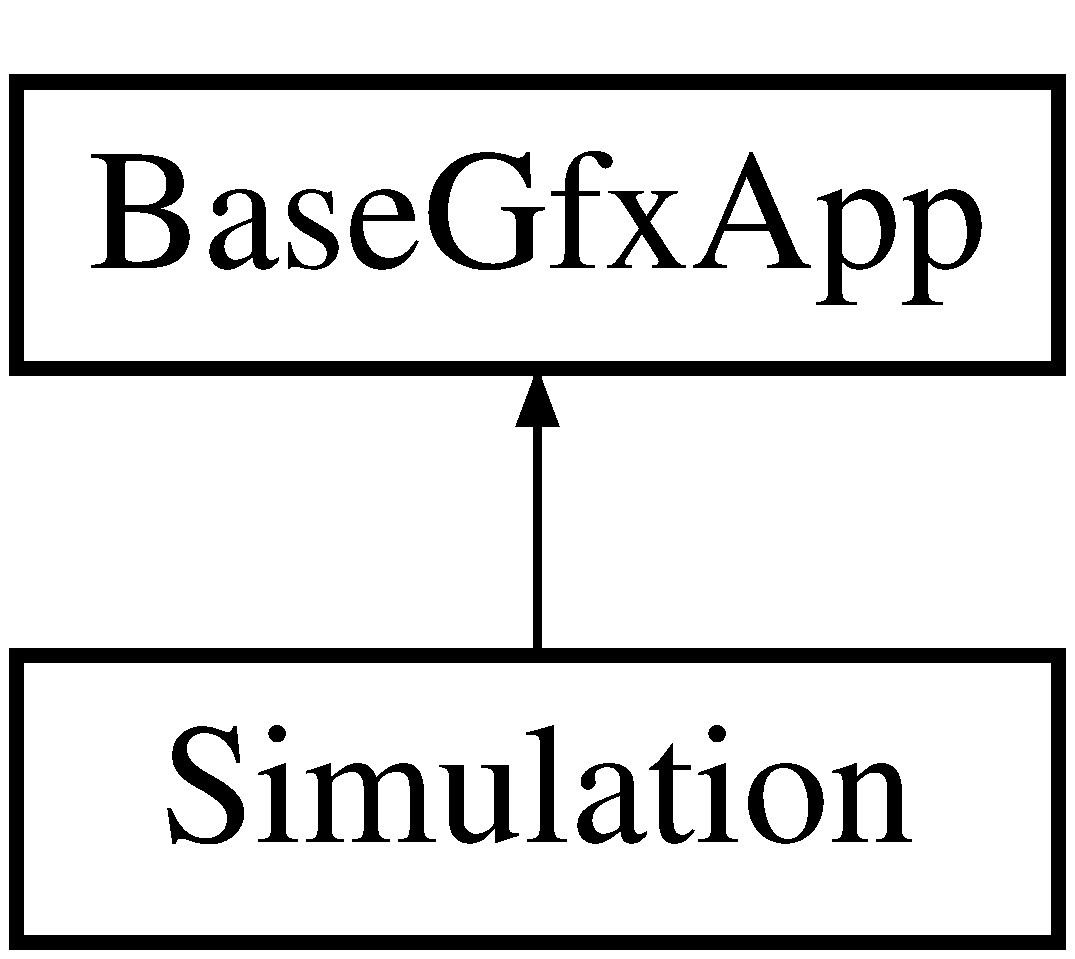
\includegraphics[height=2.000000cm]{classBaseGfxApp}
\end{center}
\end{figure}
\subsection*{Public Member Functions}
\begin{DoxyCompactItemize}
\item 
\hypertarget{classBaseGfxApp_a534a4b5293a35947fdae3805a103541d}{{\bfseries Base\+Gfx\+App} (int argc, char $\ast$argv\mbox{[}$\,$\mbox{]}, int width, int height, int x, int y, int glut\+Flags, bool create\+G\+L\+U\+I\+Win, int glui\+Win\+X, int glui\+Win\+Y)}\label{classBaseGfxApp_a534a4b5293a35947fdae3805a103541d}

\item 
\hypertarget{classBaseGfxApp_a4b3b1a475b7f2babaf1b477c34b15fb1}{void {\bfseries set\+Caption} (const std\+::string \&caption)}\label{classBaseGfxApp_a4b3b1a475b7f2babaf1b477c34b15fb1}

\item 
\hypertarget{classBaseGfxApp_acda031916c00d56c2dc901e2653e3083}{void {\bfseries run\+Main\+Loop} ()}\label{classBaseGfxApp_acda031916c00d56c2dc901e2653e3083}

\item 
\hypertarget{classBaseGfxApp_ac8de2d5a955582547af5619b771b4d6d}{virtual void {\bfseries display} ()}\label{classBaseGfxApp_ac8de2d5a955582547af5619b771b4d6d}

\item 
\hypertarget{classBaseGfxApp_a0956b82d7fa58b623c498aea7073dbba}{virtual void {\bfseries mouse\+Moved} (int x, int y)}\label{classBaseGfxApp_a0956b82d7fa58b623c498aea7073dbba}

\item 
\hypertarget{classBaseGfxApp_abb23f716dd6612b3a72938e41525d338}{virtual void {\bfseries mouse\+Dragged} (int x, int y)}\label{classBaseGfxApp_abb23f716dd6612b3a72938e41525d338}

\item 
\hypertarget{classBaseGfxApp_aaaccf5a5e923a9465441a5ee712424a8}{virtual void {\bfseries left\+Mouse\+Down} (int x, int y)}\label{classBaseGfxApp_aaaccf5a5e923a9465441a5ee712424a8}

\item 
\hypertarget{classBaseGfxApp_a0a2961a932b02b2f9d7d0bb408f6fb51}{virtual void {\bfseries left\+Mouse\+Up} (int x, int y)}\label{classBaseGfxApp_a0a2961a932b02b2f9d7d0bb408f6fb51}

\item 
\hypertarget{classBaseGfxApp_afa87e6a71220945e41f0424e540125d9}{virtual void {\bfseries right\+Mouse\+Down} (int x, int y)}\label{classBaseGfxApp_afa87e6a71220945e41f0424e540125d9}

\item 
\hypertarget{classBaseGfxApp_a812643d563522a993457dd565c33f8f6}{virtual void {\bfseries right\+Mouse\+Up} (int x, int y)}\label{classBaseGfxApp_a812643d563522a993457dd565c33f8f6}

\item 
\hypertarget{classBaseGfxApp_a2c98cae9bb5ad1fb1832a6d4812670f8}{virtual void {\bfseries middle\+Mouse\+Down} (int x, int y)}\label{classBaseGfxApp_a2c98cae9bb5ad1fb1832a6d4812670f8}

\item 
\hypertarget{classBaseGfxApp_a00fc05e8d9629b72302b5adf014bdb0c}{virtual void {\bfseries middle\+Mouse\+Up} (int x, int y)}\label{classBaseGfxApp_a00fc05e8d9629b72302b5adf014bdb0c}

\item 
\hypertarget{classBaseGfxApp_a6d91e0cb7a3d48cad33956efe7eb36ca}{virtual void {\bfseries keyboard} (unsigned char c, int x, int y)}\label{classBaseGfxApp_a6d91e0cb7a3d48cad33956efe7eb36ca}

\item 
\hypertarget{classBaseGfxApp_a345566e62c9e4ec3705ec4d1c4c75f1f}{virtual void {\bfseries keyboard\+Special} (int key, int x, int y)}\label{classBaseGfxApp_a345566e62c9e4ec3705ec4d1c4c75f1f}

\item 
\hypertarget{classBaseGfxApp_acc4a40ce11edd6b6660a19cb4802a2bf}{virtual void {\bfseries keyboard\+Up} (unsigned char c, int x, int y)}\label{classBaseGfxApp_acc4a40ce11edd6b6660a19cb4802a2bf}

\item 
\hypertarget{classBaseGfxApp_afd14b435ff93b1e7f461cb8bd1a6fd59}{virtual void {\bfseries keyboard\+Special\+Up} (int key, int x, int y)}\label{classBaseGfxApp_afd14b435ff93b1e7f461cb8bd1a6fd59}

\item 
\hypertarget{classBaseGfxApp_a5d8d5d778a8aecd7f5f8e9c87f4c3d20}{virtual void {\bfseries reshape} (int width, int height)}\label{classBaseGfxApp_a5d8d5d778a8aecd7f5f8e9c87f4c3d20}

\item 
\hypertarget{classBaseGfxApp_a2978a7c358794c67df73b66776b2cef3}{virtual void {\bfseries glui\+Control} (int control\+I\+D)}\label{classBaseGfxApp_a2978a7c358794c67df73b66776b2cef3}

\item 
\hypertarget{classBaseGfxApp_ace089a1a94fb6bb0bc17e1b7fa48e05d}{int {\bfseries width} () const }\label{classBaseGfxApp_ace089a1a94fb6bb0bc17e1b7fa48e05d}

\item 
\hypertarget{classBaseGfxApp_aa253dbe16a20c40e0a1bf8ff942ceea3}{int {\bfseries height} () const }\label{classBaseGfxApp_aa253dbe16a20c40e0a1bf8ff942ceea3}

\item 
\hypertarget{classBaseGfxApp_ae9779f948eff6f45beec08091e98a803}{int {\bfseries handle} ()}\label{classBaseGfxApp_ae9779f948eff6f45beec08091e98a803}

\item 
\hypertarget{classBaseGfxApp_ac721a0fedce80308c5c0e5695016e95d}{G\+L\+U\+I $\ast$ {\bfseries glui} ()}\label{classBaseGfxApp_ac721a0fedce80308c5c0e5695016e95d}

\end{DoxyCompactItemize}
\subsection*{Static Protected Member Functions}
\begin{DoxyCompactItemize}
\item 
\hypertarget{classBaseGfxApp_a5fe6a77d37044cbe28647ed3391bbb7a}{static void {\bfseries s\+\_\+reshape} (int width, int height)}\label{classBaseGfxApp_a5fe6a77d37044cbe28647ed3391bbb7a}

\item 
\hypertarget{classBaseGfxApp_a52edb2569227319feb68779844e7d857}{static void {\bfseries s\+\_\+keyboard} (unsigned char c, int x, int y)}\label{classBaseGfxApp_a52edb2569227319feb68779844e7d857}

\item 
\hypertarget{classBaseGfxApp_a1e8d90a4faab60300ddf2a4ea9b83115}{static void {\bfseries s\+\_\+keyboardspecial} (int key, int x, int y)}\label{classBaseGfxApp_a1e8d90a4faab60300ddf2a4ea9b83115}

\item 
\hypertarget{classBaseGfxApp_aa1ca205af9d6cee33949f2e6adf4c923}{static void {\bfseries s\+\_\+keyboardup} (unsigned char c, int x, int y)}\label{classBaseGfxApp_aa1ca205af9d6cee33949f2e6adf4c923}

\item 
\hypertarget{classBaseGfxApp_a0e4dfe006f3cc9126c1cc8ad32784f75}{static void {\bfseries s\+\_\+keyboardspecialup} (int key, int x, int y)}\label{classBaseGfxApp_a0e4dfe006f3cc9126c1cc8ad32784f75}

\item 
\hypertarget{classBaseGfxApp_a5e640f2394f7e038d0dd2b469d5c2e24}{static void {\bfseries s\+\_\+mousemotion} (int x, int y)}\label{classBaseGfxApp_a5e640f2394f7e038d0dd2b469d5c2e24}

\item 
\hypertarget{classBaseGfxApp_a22dd953bfb75add9fd0f8f2f8be535c5}{static void {\bfseries s\+\_\+mousebtn} (int b, int s, int x, int y)}\label{classBaseGfxApp_a22dd953bfb75add9fd0f8f2f8be535c5}

\item 
\hypertarget{classBaseGfxApp_a58415c6151a2a80e1fe2eaa9919a4dab}{static void {\bfseries s\+\_\+draw} ()}\label{classBaseGfxApp_a58415c6151a2a80e1fe2eaa9919a4dab}

\item 
\hypertarget{classBaseGfxApp_ad4a963321f1147d68369225ab0c7f32f}{static void {\bfseries s\+\_\+gluicallback} (int control\+I\+D)}\label{classBaseGfxApp_ad4a963321f1147d68369225ab0c7f32f}

\end{DoxyCompactItemize}
\subsection*{Protected Attributes}
\begin{DoxyCompactItemize}
\item 
int \hyperlink{classBaseGfxApp_ad8697d6fdd10e6f336c3a662016b4fa7}{m\+\_\+glut\+Window\+Handle}
\item 
\hypertarget{classBaseGfxApp_a6eb1673b80283727221da2242211af1d}{G\+L\+U\+I $\ast$ {\bfseries m\+\_\+glui}}\label{classBaseGfxApp_a6eb1673b80283727221da2242211af1d}

\item 
\hypertarget{classBaseGfxApp_a2e70a389224f8affe7c137f7e20dc8c1}{bool {\bfseries m\+\_\+drag}}\label{classBaseGfxApp_a2e70a389224f8affe7c137f7e20dc8c1}

\item 
\hypertarget{classBaseGfxApp_a7e5ef1c8f25fe081b4a1fd4ce6a96e07}{int {\bfseries m\+\_\+width}}\label{classBaseGfxApp_a7e5ef1c8f25fe081b4a1fd4ce6a96e07}

\item 
\hypertarget{classBaseGfxApp_ac078e4fc20b5c2fe0c744966b850b412}{int {\bfseries m\+\_\+height}}\label{classBaseGfxApp_ac078e4fc20b5c2fe0c744966b850b412}

\end{DoxyCompactItemize}
\subsection*{Static Protected Attributes}
\begin{DoxyCompactItemize}
\item 
static \hyperlink{classBaseGfxApp}{Base\+Gfx\+App} $\ast$ \hyperlink{classBaseGfxApp_a65ba89b98af31e2649a0546631931000}{s\+\_\+current\+App} = N\+U\+L\+L
\item 
static bool \hyperlink{classBaseGfxApp_afa4690383ea27713016ef75b9fb1e42f}{s\+\_\+glut\+Initialized} = false
\end{DoxyCompactItemize}


\subsection{Member Data Documentation}
\hypertarget{classBaseGfxApp_ad8697d6fdd10e6f336c3a662016b4fa7}{\index{Base\+Gfx\+App@{Base\+Gfx\+App}!m\+\_\+glut\+Window\+Handle@{m\+\_\+glut\+Window\+Handle}}
\index{m\+\_\+glut\+Window\+Handle@{m\+\_\+glut\+Window\+Handle}!Base\+Gfx\+App@{Base\+Gfx\+App}}
\subsubsection[{m\+\_\+glut\+Window\+Handle}]{\setlength{\rightskip}{0pt plus 5cm}int Base\+Gfx\+App\+::m\+\_\+glut\+Window\+Handle\hspace{0.3cm}{\ttfamily [protected]}}}\label{classBaseGfxApp_ad8697d6fdd10e6f336c3a662016b4fa7}
Underlying glut window handle \hypertarget{classBaseGfxApp_a65ba89b98af31e2649a0546631931000}{\index{Base\+Gfx\+App@{Base\+Gfx\+App}!s\+\_\+current\+App@{s\+\_\+current\+App}}
\index{s\+\_\+current\+App@{s\+\_\+current\+App}!Base\+Gfx\+App@{Base\+Gfx\+App}}
\subsubsection[{s\+\_\+current\+App}]{\setlength{\rightskip}{0pt plus 5cm}{\bf Base\+Gfx\+App} $\ast$ Base\+Gfx\+App\+::s\+\_\+current\+App = N\+U\+L\+L\hspace{0.3cm}{\ttfamily [static]}, {\ttfamily [protected]}}}\label{classBaseGfxApp_a65ba89b98af31e2649a0546631931000}
G\+L\+U\+T and G\+L\+U\+I event callbacks are sent to the current window/app. Right now, there is only one window anyway (not counting the G\+L\+U\+I U\+I window.. in the future could be extended to support more windows. In any case, some structure like this is always needed when using glut with C++, since the glut callbacks must be either global or static functions. \hypertarget{classBaseGfxApp_afa4690383ea27713016ef75b9fb1e42f}{\index{Base\+Gfx\+App@{Base\+Gfx\+App}!s\+\_\+glut\+Initialized@{s\+\_\+glut\+Initialized}}
\index{s\+\_\+glut\+Initialized@{s\+\_\+glut\+Initialized}!Base\+Gfx\+App@{Base\+Gfx\+App}}
\subsubsection[{s\+\_\+glut\+Initialized}]{\setlength{\rightskip}{0pt plus 5cm}bool Base\+Gfx\+App\+::s\+\_\+glut\+Initialized = false\hspace{0.3cm}{\ttfamily [static]}, {\ttfamily [protected]}}}\label{classBaseGfxApp_afa4690383ea27713016ef75b9fb1e42f}
Has glut\+Init been called? (only allowed once per program) 

The documentation for this class was generated from the following files\+:\begin{DoxyCompactItemize}
\item 
\hyperlink{BaseGfxApp_8h}{Base\+Gfx\+App.\+h}\item 
Base\+Gfx\+App.\+cpp\end{DoxyCompactItemize}

\hypertarget{classPlayer}{\section{Player Class Reference}
\label{classPlayer}\index{Player@{Player}}
}


The \hyperlink{classPlayer}{Player} class. This sets up player and paddle.  




{\ttfamily \#include $<$Player.\+h$>$}

\subsection*{Public Member Functions}
\begin{DoxyCompactItemize}
\item 
\hyperlink{classPlayer_a8b3405e45f13fe028bc6d8b5d4858c61}{Player} (float x, float y, float l, float w, float ori, float sp)
\begin{DoxyCompactList}\small\item\em Constructor. \end{DoxyCompactList}\item 
\hypertarget{classPlayer_a749d2c00e1fe0f5c2746f7505a58c062}{\hyperlink{classPlayer_a749d2c00e1fe0f5c2746f7505a58c062}{$\sim$\+Player} ()}\label{classPlayer_a749d2c00e1fe0f5c2746f7505a58c062}

\begin{DoxyCompactList}\small\item\em Default Constructor. \end{DoxyCompactList}\item 
void \hyperlink{classPlayer_a3d91e6c646470b645bdb302318ba9998}{set\+X\+Position} (float new\+X)
\begin{DoxyCompactList}\small\item\em Mutator to change the x position of the paddle according to the input. \end{DoxyCompactList}\item 
void \hyperlink{classPlayer_a593a81af1e971fa6410f5ee980ac0c0e}{set\+Y\+Position} (float new\+Y)
\begin{DoxyCompactList}\small\item\em Mutator to change the x position of the paddle according to the input. \end{DoxyCompactList}\item 
void \hyperlink{classPlayer_a7fbd49a140da0e4c40122040456d3542}{set\+Length} (float l)
\begin{DoxyCompactList}\small\item\em Mutator to change the length of the paddle according to the input. \end{DoxyCompactList}\item 
void \hyperlink{classPlayer_a2c37171e8a3aafcedb8f89127d77ed03}{set\+Width} (float w)
\begin{DoxyCompactList}\small\item\em Mutator to change the width of the paddle according to the input. \end{DoxyCompactList}\item 
void \hyperlink{classPlayer_a3bd54fb199f66e8320b1204c75cf10f3}{set\+Speed} (float sp)
\begin{DoxyCompactList}\small\item\em set paddle's speed through arguement. \end{DoxyCompactList}\item 
void \hyperlink{classPlayer_ad7b5956c42a1ce32c536f4ac436ff10d}{set\+Orientation} (float ori)
\begin{DoxyCompactList}\small\item\em Mutator to change the orientation of the paddle according to the input. \end{DoxyCompactList}\item 
\hypertarget{classPlayer_a60127b852551bc42cdd0ad3a5ce84c39}{float \hyperlink{classPlayer_a60127b852551bc42cdd0ad3a5ce84c39}{get\+X\+Position} ()}\label{classPlayer_a60127b852551bc42cdd0ad3a5ce84c39}

\begin{DoxyCompactList}\small\item\em Getter to get the x position of the paddle. \end{DoxyCompactList}\item 
\hypertarget{classPlayer_adb0156f686b1aa98f74dc8db0d6305ee}{float \hyperlink{classPlayer_adb0156f686b1aa98f74dc8db0d6305ee}{get\+Y\+Position} ()}\label{classPlayer_adb0156f686b1aa98f74dc8db0d6305ee}

\begin{DoxyCompactList}\small\item\em Getter to get the y position of the paddle. \end{DoxyCompactList}\item 
\hypertarget{classPlayer_ae10f3a8d97b0a6fa3a3a6761c0337ab7}{float \hyperlink{classPlayer_ae10f3a8d97b0a6fa3a3a6761c0337ab7}{get\+Length} ()}\label{classPlayer_ae10f3a8d97b0a6fa3a3a6761c0337ab7}

\begin{DoxyCompactList}\small\item\em Getter to get the Length of the paddle. \end{DoxyCompactList}\item 
\hypertarget{classPlayer_a5317c44d9a85a1b25435edf74c0994e9}{float \hyperlink{classPlayer_a5317c44d9a85a1b25435edf74c0994e9}{get\+Width} ()}\label{classPlayer_a5317c44d9a85a1b25435edf74c0994e9}

\begin{DoxyCompactList}\small\item\em Getter to get the Width of the paddle. \end{DoxyCompactList}\item 
\hypertarget{classPlayer_aeb38adafb5e2ef723021225410e20668}{float \hyperlink{classPlayer_aeb38adafb5e2ef723021225410e20668}{get\+Orientation} ()}\label{classPlayer_aeb38adafb5e2ef723021225410e20668}

\begin{DoxyCompactList}\small\item\em Getter to get the position of the paddle. \end{DoxyCompactList}\item 
\hypertarget{classPlayer_a63caffe9c0cbb3b776811ad45a545aa9}{float \hyperlink{classPlayer_a63caffe9c0cbb3b776811ad45a545aa9}{get\+Speed} ()}\label{classPlayer_a63caffe9c0cbb3b776811ad45a545aa9}

\begin{DoxyCompactList}\small\item\em Getter to get the speed of the paddle. \end{DoxyCompactList}\item 
void \hyperlink{classPlayer_a981b84ed6dba35c941685b74c8ca5feb}{move} (int w, int h)
\begin{DoxyCompactList}\small\item\em Move the Paddle accoding to the step time and speed. \end{DoxyCompactList}\end{DoxyCompactItemize}


\subsection{Detailed Description}
The \hyperlink{classPlayer}{Player} class. This sets up player and paddle. 

\subsection{Constructor \& Destructor Documentation}
\hypertarget{classPlayer_a8b3405e45f13fe028bc6d8b5d4858c61}{\index{Player@{Player}!Player@{Player}}
\index{Player@{Player}!Player@{Player}}
\subsubsection[{Player}]{\setlength{\rightskip}{0pt plus 5cm}Player\+::\+Player (
\begin{DoxyParamCaption}
\item[{float}]{x, }
\item[{float}]{y, }
\item[{float}]{l, }
\item[{float}]{w, }
\item[{float}]{ori, }
\item[{float}]{sp}
\end{DoxyParamCaption}
)}}\label{classPlayer_a8b3405e45f13fe028bc6d8b5d4858c61}


Constructor. 


\begin{DoxyParams}{Parameters}
{\em x} & The center x position of paddle. \\
\hline
{\em y} & The center y position of paddle. \\
\hline
{\em l} & The length of paddle. \\
\hline
{\em w} & The width of paddle. \\
\hline
{\em ori} & The orientation of paddle. \\
\hline
{\em sp} & The speed of paddle. \\
\hline
\end{DoxyParams}


\subsection{Member Function Documentation}
\hypertarget{classPlayer_a981b84ed6dba35c941685b74c8ca5feb}{\index{Player@{Player}!move@{move}}
\index{move@{move}!Player@{Player}}
\subsubsection[{move}]{\setlength{\rightskip}{0pt plus 5cm}void Player\+::move (
\begin{DoxyParamCaption}
\item[{int}]{w, }
\item[{int}]{h}
\end{DoxyParamCaption}
)}}\label{classPlayer_a981b84ed6dba35c941685b74c8ca5feb}


Move the Paddle accoding to the step time and speed. 


\begin{DoxyParams}{Parameters}
{\em w} & The witdth of window(default\+: 800) \\
\hline
{\em h} & The height of window(default\+: 800) \\
\hline
\end{DoxyParams}
\hypertarget{classPlayer_a7fbd49a140da0e4c40122040456d3542}{\index{Player@{Player}!set\+Length@{set\+Length}}
\index{set\+Length@{set\+Length}!Player@{Player}}
\subsubsection[{set\+Length}]{\setlength{\rightskip}{0pt plus 5cm}void Player\+::set\+Length (
\begin{DoxyParamCaption}
\item[{float}]{l}
\end{DoxyParamCaption}
)}}\label{classPlayer_a7fbd49a140da0e4c40122040456d3542}


Mutator to change the length of the paddle according to the input. 


\begin{DoxyParams}{Parameters}
{\em l} & The new length value. \\
\hline
\end{DoxyParams}
\hypertarget{classPlayer_ad7b5956c42a1ce32c536f4ac436ff10d}{\index{Player@{Player}!set\+Orientation@{set\+Orientation}}
\index{set\+Orientation@{set\+Orientation}!Player@{Player}}
\subsubsection[{set\+Orientation}]{\setlength{\rightskip}{0pt plus 5cm}void Player\+::set\+Orientation (
\begin{DoxyParamCaption}
\item[{float}]{ori}
\end{DoxyParamCaption}
)}}\label{classPlayer_ad7b5956c42a1ce32c536f4ac436ff10d}


Mutator to change the orientation of the paddle according to the input. 


\begin{DoxyParams}{Parameters}
{\em new\+X} & The new orientation value. \\
\hline
\end{DoxyParams}
\hypertarget{classPlayer_a3bd54fb199f66e8320b1204c75cf10f3}{\index{Player@{Player}!set\+Speed@{set\+Speed}}
\index{set\+Speed@{set\+Speed}!Player@{Player}}
\subsubsection[{set\+Speed}]{\setlength{\rightskip}{0pt plus 5cm}void Player\+::set\+Speed (
\begin{DoxyParamCaption}
\item[{float}]{sp}
\end{DoxyParamCaption}
)}}\label{classPlayer_a3bd54fb199f66e8320b1204c75cf10f3}


set paddle's speed through arguement. 


\begin{DoxyParams}{Parameters}
{\em sp} & Set paddle's speed according to arguement double sp. \\
\hline
\end{DoxyParams}
\hypertarget{classPlayer_a2c37171e8a3aafcedb8f89127d77ed03}{\index{Player@{Player}!set\+Width@{set\+Width}}
\index{set\+Width@{set\+Width}!Player@{Player}}
\subsubsection[{set\+Width}]{\setlength{\rightskip}{0pt plus 5cm}void Player\+::set\+Width (
\begin{DoxyParamCaption}
\item[{float}]{w}
\end{DoxyParamCaption}
)}}\label{classPlayer_a2c37171e8a3aafcedb8f89127d77ed03}


Mutator to change the width of the paddle according to the input. 


\begin{DoxyParams}{Parameters}
{\em l} & The new length value. \\
\hline
\end{DoxyParams}
\hypertarget{classPlayer_a3d91e6c646470b645bdb302318ba9998}{\index{Player@{Player}!set\+X\+Position@{set\+X\+Position}}
\index{set\+X\+Position@{set\+X\+Position}!Player@{Player}}
\subsubsection[{set\+X\+Position}]{\setlength{\rightskip}{0pt plus 5cm}void Player\+::set\+X\+Position (
\begin{DoxyParamCaption}
\item[{float}]{new\+X}
\end{DoxyParamCaption}
)}}\label{classPlayer_a3d91e6c646470b645bdb302318ba9998}


Mutator to change the x position of the paddle according to the input. 


\begin{DoxyParams}{Parameters}
{\em new\+X} & The new X position value. \\
\hline
\end{DoxyParams}
\hypertarget{classPlayer_a593a81af1e971fa6410f5ee980ac0c0e}{\index{Player@{Player}!set\+Y\+Position@{set\+Y\+Position}}
\index{set\+Y\+Position@{set\+Y\+Position}!Player@{Player}}
\subsubsection[{set\+Y\+Position}]{\setlength{\rightskip}{0pt plus 5cm}void Player\+::set\+Y\+Position (
\begin{DoxyParamCaption}
\item[{float}]{new\+Y}
\end{DoxyParamCaption}
)}}\label{classPlayer_a593a81af1e971fa6410f5ee980ac0c0e}


Mutator to change the x position of the paddle according to the input. 


\begin{DoxyParams}{Parameters}
{\em new\+X} & The new X position value. \\
\hline
\end{DoxyParams}


The documentation for this class was generated from the following files\+:\begin{DoxyCompactItemize}
\item 
\hyperlink{Player_8h}{Player.\+h}\item 
\hyperlink{Player_8cpp}{Player.\+cpp}\end{DoxyCompactItemize}

\hypertarget{classPongGame}{\section{Pong\+Game Class Reference}
\label{classPongGame}\index{Pong\+Game@{Pong\+Game}}
}


The \hyperlink{classPongGame}{Pong\+Game} class. This class represents game environment.  




{\ttfamily \#include $<$Pong\+Game.\+h$>$}

\subsection*{Public Member Functions}
\begin{DoxyCompactItemize}
\item 
\hyperlink{classPongGame_ab43c680542f00834d51ad75da21e5b4f}{Pong\+Game} (int width, int height, std\+::vector$<$ \hyperlink{classBall}{Ball} $>$ $\ast$b, std\+::vector$<$ \hyperlink{classPlayer}{Player} $>$ $\ast$p)
\begin{DoxyCompactList}\small\item\em Constructor. \end{DoxyCompactList}\item 
\hypertarget{classPongGame_afb95a66cbc5618ca9c73476f8c51ab94}{\hyperlink{classPongGame_afb95a66cbc5618ca9c73476f8c51ab94}{$\sim$\+Pong\+Game} ()}\label{classPongGame_afb95a66cbc5618ca9c73476f8c51ab94}

\begin{DoxyCompactList}\small\item\em Default Constructor. \end{DoxyCompactList}\item 
int \hyperlink{classPongGame_ad5ced36934c6597e1ba0603108953826}{update\+Move} ()
\begin{DoxyCompactList}\small\item\em Update the status of game by the specificied amount time. \end{DoxyCompactList}\item 
void \hyperlink{classPongGame_a10d3179a962692fef5bda0dc9927d368}{register\+Ball} (\hyperlink{classBall}{Ball} b)
\begin{DoxyCompactList}\small\item\em Balls register with the environment, which adds them to the environment data structure(s). \end{DoxyCompactList}\item 
void \hyperlink{classPongGame_a8372b9946c95954b35fcf4c3543c11c2}{register\+Player} (\hyperlink{classPlayer}{Player} p)
\begin{DoxyCompactList}\small\item\em Players register with the environment, which adds them to the environment data structure(s). \end{DoxyCompactList}\item 
\hypertarget{classPongGame_a911a5071f520fd9989b9b4de2039c982}{void \hyperlink{classPongGame_a911a5071f520fd9989b9b4de2039c982}{Start\+New\+Game} ()}\label{classPongGame_a911a5071f520fd9989b9b4de2039c982}

\begin{DoxyCompactList}\small\item\em Start a new Game. \end{DoxyCompactList}\item 
\hypertarget{classPongGame_aa920817372d5aa5f8309ceb6b10d3a5e}{time\+\_\+t \hyperlink{classPongGame_aa920817372d5aa5f8309ceb6b10d3a5e}{get\+Start\+Time} ()}\label{classPongGame_aa920817372d5aa5f8309ceb6b10d3a5e}

\begin{DoxyCompactList}\small\item\em Getter to get the start time of the game. \end{DoxyCompactList}\item 
\hypertarget{classPongGame_aa96aa2608d7c211319175857faf3dbf6}{double \hyperlink{classPongGame_aa96aa2608d7c211319175857faf3dbf6}{get\+Difftime} ()}\label{classPongGame_aa96aa2608d7c211319175857faf3dbf6}

\begin{DoxyCompactList}\small\item\em Getter to get the how long does game last. \end{DoxyCompactList}\item 
int \hyperlink{classPongGame_acf5bed550d45e295b7ba231f5c77f8b7}{get\+Scorei} (int i)
\begin{DoxyCompactList}\small\item\em Getter to get the specific score according to the input index. \end{DoxyCompactList}\item 
\hypertarget{classPongGame_afa96567179aa1748c3fb63ed83524ccb}{int \hyperlink{classPongGame_afa96567179aa1748c3fb63ed83524ccb}{get\+Mode} ()}\label{classPongGame_afa96567179aa1748c3fb63ed83524ccb}

\begin{DoxyCompactList}\small\item\em Getter to get the mode of game. \end{DoxyCompactList}\item 
void \hyperlink{classPongGame_a15649211e81c19c363c1b37be73d4d90}{set\+Start\+Time} (time\+\_\+t new\+Time)
\begin{DoxyCompactList}\small\item\em Mutator to change the start time of the game. \end{DoxyCompactList}\item 
void \hyperlink{classPongGame_a0e74f3db80283de1fae5a018f6e62f35}{set\+Mode} (int i)
\begin{DoxyCompactList}\small\item\em Mutator to change the mode of the game. \end{DoxyCompactList}\item 
void \hyperlink{classPongGame_ac4f09e4632cfda46521fdce2fe0f7167}{set\+Difftime} (double newdiff\+Time)
\begin{DoxyCompactList}\small\item\em Mutator to change lasting time of the game. \end{DoxyCompactList}\end{DoxyCompactItemize}


\subsection{Detailed Description}
The \hyperlink{classPongGame}{Pong\+Game} class. This class represents game environment. 

\subsection{Constructor \& Destructor Documentation}
\hypertarget{classPongGame_ab43c680542f00834d51ad75da21e5b4f}{\index{Pong\+Game@{Pong\+Game}!Pong\+Game@{Pong\+Game}}
\index{Pong\+Game@{Pong\+Game}!Pong\+Game@{Pong\+Game}}
\subsubsection[{Pong\+Game}]{\setlength{\rightskip}{0pt plus 5cm}Pong\+Game\+::\+Pong\+Game (
\begin{DoxyParamCaption}
\item[{int}]{w, }
\item[{int}]{h, }
\item[{std\+::vector$<$ {\bf Ball} $>$ $\ast$}]{b, }
\item[{std\+::vector$<$ {\bf Player} $>$ $\ast$}]{p}
\end{DoxyParamCaption}
)}}\label{classPongGame_ab43c680542f00834d51ad75da21e5b4f}


Constructor. 


\begin{DoxyParams}{Parameters}
{\em width} & The width of window. \\
\hline
{\em height} & The height of window. \\
\hline
{\em b} & The balls in the game. \\
\hline
{\em p} & The players in the game. \\
\hline
\end{DoxyParams}


\subsection{Member Function Documentation}
\hypertarget{classPongGame_acf5bed550d45e295b7ba231f5c77f8b7}{\index{Pong\+Game@{Pong\+Game}!get\+Scorei@{get\+Scorei}}
\index{get\+Scorei@{get\+Scorei}!Pong\+Game@{Pong\+Game}}
\subsubsection[{get\+Scorei}]{\setlength{\rightskip}{0pt plus 5cm}int Pong\+Game\+::get\+Scorei (
\begin{DoxyParamCaption}
\item[{int}]{i}
\end{DoxyParamCaption}
)}}\label{classPongGame_acf5bed550d45e295b7ba231f5c77f8b7}


Getter to get the specific score according to the input index. 


\begin{DoxyParams}{Parameters}
{\em i} & The index of the specific score. \\
\hline
\end{DoxyParams}
\hypertarget{classPongGame_a10d3179a962692fef5bda0dc9927d368}{\index{Pong\+Game@{Pong\+Game}!register\+Ball@{register\+Ball}}
\index{register\+Ball@{register\+Ball}!Pong\+Game@{Pong\+Game}}
\subsubsection[{register\+Ball}]{\setlength{\rightskip}{0pt plus 5cm}void Pong\+Game\+::register\+Ball (
\begin{DoxyParamCaption}
\item[{{\bf Ball}}]{b}
\end{DoxyParamCaption}
)}}\label{classPongGame_a10d3179a962692fef5bda0dc9927d368}


Balls register with the environment, which adds them to the environment data structure(s). 


\begin{DoxyParams}{Parameters}
{\em b} & the ball need to be registered to the environment. \\
\hline
\end{DoxyParams}
\hypertarget{classPongGame_a8372b9946c95954b35fcf4c3543c11c2}{\index{Pong\+Game@{Pong\+Game}!register\+Player@{register\+Player}}
\index{register\+Player@{register\+Player}!Pong\+Game@{Pong\+Game}}
\subsubsection[{register\+Player}]{\setlength{\rightskip}{0pt plus 5cm}void Pong\+Game\+::register\+Player (
\begin{DoxyParamCaption}
\item[{{\bf Player}}]{p}
\end{DoxyParamCaption}
)}}\label{classPongGame_a8372b9946c95954b35fcf4c3543c11c2}


Players register with the environment, which adds them to the environment data structure(s). 


\begin{DoxyParams}{Parameters}
{\em p} & the player need to be registered to the environment. \\
\hline
\end{DoxyParams}
\hypertarget{classPongGame_ac4f09e4632cfda46521fdce2fe0f7167}{\index{Pong\+Game@{Pong\+Game}!set\+Difftime@{set\+Difftime}}
\index{set\+Difftime@{set\+Difftime}!Pong\+Game@{Pong\+Game}}
\subsubsection[{set\+Difftime}]{\setlength{\rightskip}{0pt plus 5cm}void Pong\+Game\+::set\+Difftime (
\begin{DoxyParamCaption}
\item[{double}]{newdiff\+Time}
\end{DoxyParamCaption}
)}}\label{classPongGame_ac4f09e4632cfda46521fdce2fe0f7167}


Mutator to change lasting time of the game. 


\begin{DoxyParams}{Parameters}
{\em newdiff\+Time} & The lasting time of the game. \\
\hline
\end{DoxyParams}
\hypertarget{classPongGame_a0e74f3db80283de1fae5a018f6e62f35}{\index{Pong\+Game@{Pong\+Game}!set\+Mode@{set\+Mode}}
\index{set\+Mode@{set\+Mode}!Pong\+Game@{Pong\+Game}}
\subsubsection[{set\+Mode}]{\setlength{\rightskip}{0pt plus 5cm}void Pong\+Game\+::set\+Mode (
\begin{DoxyParamCaption}
\item[{int}]{i}
\end{DoxyParamCaption}
)}}\label{classPongGame_a0e74f3db80283de1fae5a018f6e62f35}


Mutator to change the mode of the game. 


\begin{DoxyParams}{Parameters}
{\em i} & The mode of the game. \\
\hline
\end{DoxyParams}
\hypertarget{classPongGame_a15649211e81c19c363c1b37be73d4d90}{\index{Pong\+Game@{Pong\+Game}!set\+Start\+Time@{set\+Start\+Time}}
\index{set\+Start\+Time@{set\+Start\+Time}!Pong\+Game@{Pong\+Game}}
\subsubsection[{set\+Start\+Time}]{\setlength{\rightskip}{0pt plus 5cm}void Pong\+Game\+::set\+Start\+Time (
\begin{DoxyParamCaption}
\item[{time\+\_\+t}]{new\+Time}
\end{DoxyParamCaption}
)}}\label{classPongGame_a15649211e81c19c363c1b37be73d4d90}


Mutator to change the start time of the game. 


\begin{DoxyParams}{Parameters}
{\em new\+Time} & The start time of the game. \\
\hline
\end{DoxyParams}
\hypertarget{classPongGame_ad5ced36934c6597e1ba0603108953826}{\index{Pong\+Game@{Pong\+Game}!update\+Move@{update\+Move}}
\index{update\+Move@{update\+Move}!Pong\+Game@{Pong\+Game}}
\subsubsection[{update\+Move}]{\setlength{\rightskip}{0pt plus 5cm}int Pong\+Game\+::update\+Move (
\begin{DoxyParamCaption}
{}
\end{DoxyParamCaption}
)}}\label{classPongGame_ad5ced36934c6597e1ba0603108953826}


Update the status of game by the specificied amount time. 


\begin{DoxyParams}{Parameters}
{\em elasped\+Time} & The delta time. \\
\hline
\end{DoxyParams}


The documentation for this class was generated from the following files\+:\begin{DoxyCompactItemize}
\item 
\hyperlink{PongGame_8h}{Pong\+Game.\+h}\item 
\hyperlink{PongGame_8cpp}{Pong\+Game.\+cpp}\end{DoxyCompactItemize}

\hypertarget{classSimulation}{\section{Simulation Class Reference}
\label{classSimulation}\index{Simulation@{Simulation}}
}


The \hyperlink{classSimulation}{Simulation} class. This sets up the G\+U\+I and the drawing environment.  




{\ttfamily \#include $<$Simulation.\+h$>$}

Inheritance diagram for Simulation\+:\begin{figure}[H]
\begin{center}
\leavevmode
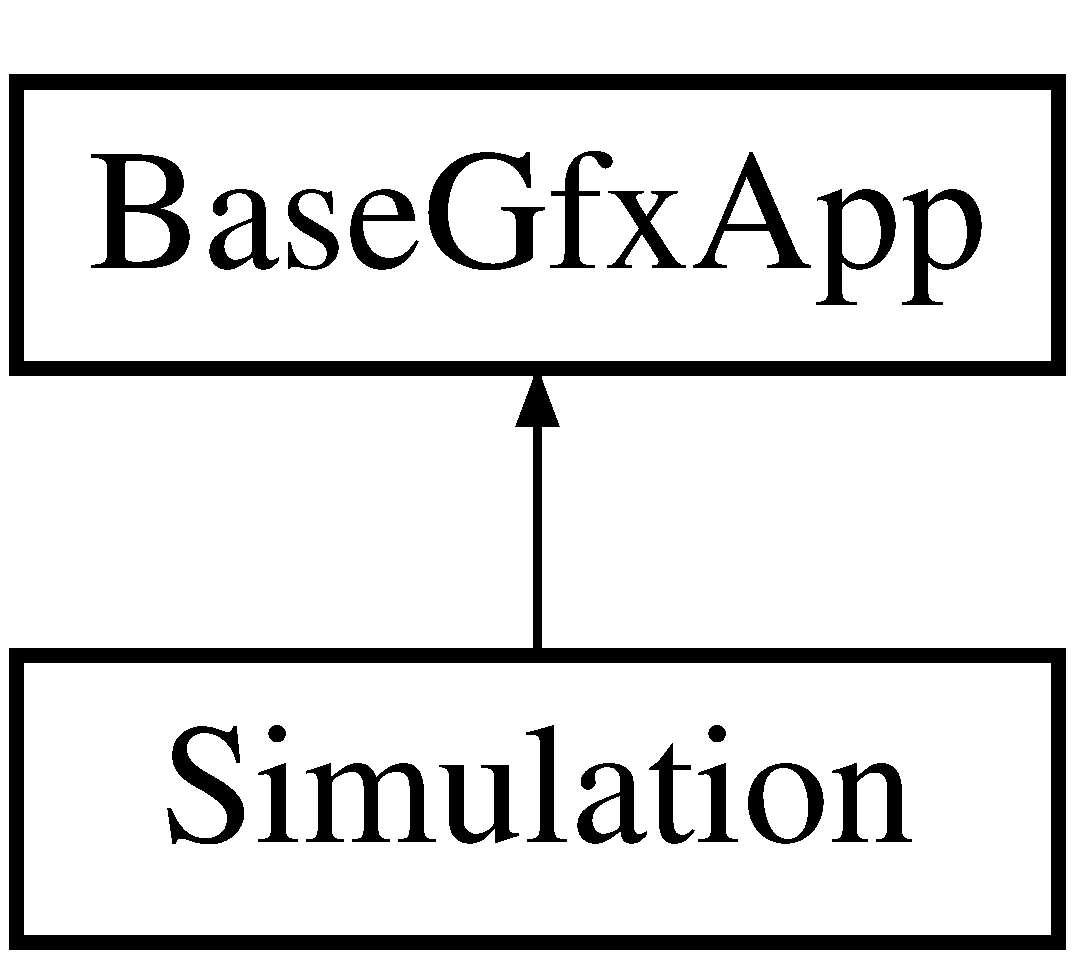
\includegraphics[height=2.000000cm]{classSimulation}
\end{center}
\end{figure}
\subsection*{Public Types}
\begin{DoxyCompactItemize}
\item 
\hypertarget{classSimulation_a0fd1c91d4e7699e893929d56b60a60bf}{enum \hyperlink{classSimulation_a0fd1c91d4e7699e893929d56b60a60bf}{U\+I\+Control\+Type} \{ \\*
{\bfseries U\+I\+\_\+\+Q\+U\+I\+T} = 0, 
{\bfseries U\+I\+\_\+\+R\+E\+S\+U\+M\+E} = 4, 
{\bfseries U\+I\+\_\+\+P\+A\+U\+S\+E} = 3, 
{\bfseries U\+I\+\_\+\+P\+R\+A\+C\+T\+I\+C\+E} = 1, 
\\*
{\bfseries U\+I\+\_\+2\+P\+L\+A\+Y\+E\+R} = 2, 
{\bfseries U\+I\+\_\+\+S\+P\+I\+N} = 5
 \}}\label{classSimulation_a0fd1c91d4e7699e893929d56b60a60bf}

\begin{DoxyCompactList}\small\item\em the type of U\+I Control input. \end{DoxyCompactList}\end{DoxyCompactItemize}
\subsection*{Public Member Functions}
\begin{DoxyCompactItemize}
\item 
\hyperlink{classSimulation_a4c669ceaa34c7130966ce45f9de75fbe}{Simulation} (int argc, char $\ast$argv\mbox{[}$\,$\mbox{]}, int width, int height)
\begin{DoxyCompactList}\small\item\em arguements from user's command input and other window information. \end{DoxyCompactList}\item 
\hypertarget{classSimulation_a80fad3f57dfaf195a36f7bc49bc88279}{virtual \hyperlink{classSimulation_a80fad3f57dfaf195a36f7bc49bc88279}{$\sim$\+Simulation} ()}\label{classSimulation_a80fad3f57dfaf195a36f7bc49bc88279}

\begin{DoxyCompactList}\small\item\em Default constructor. \end{DoxyCompactList}\item 
\hypertarget{classSimulation_a449dcb7d97dfba99efe770de2f399c31}{void \hyperlink{classSimulation_a449dcb7d97dfba99efe770de2f399c31}{display} ()}\label{classSimulation_a449dcb7d97dfba99efe770de2f399c31}

\begin{DoxyCompactList}\small\item\em display all the items. \end{DoxyCompactList}\item 
void \hyperlink{classSimulation_a1607cd18e552ab9f4a6f57d362f7121a}{glui\+Control} (int control\+I\+D)
\begin{DoxyCompactList}\small\item\em Control panel through input control id. \end{DoxyCompactList}\item 
void \hyperlink{classSimulation_aa60852eabb776ee691767c4e1e785199}{render\+Ball} (\hyperlink{classBall}{Ball} b)
\begin{DoxyCompactList}\small\item\em draw ball and send them to the window. \end{DoxyCompactList}\item 
void \hyperlink{classSimulation_a1f1da2f39bb1a8c4a5f91646e59d2480}{render\+Player} (\hyperlink{classPlayer}{Player} p)
\begin{DoxyCompactList}\small\item\em draw player and send them to the window. \end{DoxyCompactList}\item 
\hypertarget{classSimulation_a018e40e2fb25694123c4fc9999a44b64}{void \hyperlink{classSimulation_a018e40e2fb25694123c4fc9999a44b64}{render\+Score} ()}\label{classSimulation_a018e40e2fb25694123c4fc9999a44b64}

\begin{DoxyCompactList}\small\item\em draw socre and send them to the window. \end{DoxyCompactList}\item 
void \hyperlink{classSimulation_a786d1ba31d29937f0ac6f3ea88f8a607}{left\+Mouse\+Down} (int x, int y)
\begin{DoxyCompactList}\small\item\em The action will be taken when left mouse is clicked. \end{DoxyCompactList}\item 
void \hyperlink{classSimulation_a62ef254d85017074cd521a5787b5a234}{left\+Mouse\+Up} (int x, int y)
\begin{DoxyCompactList}\small\item\em The action will be taken when left mouse is released. \end{DoxyCompactList}\item 
\hypertarget{classSimulation_a6a27947a5930814ce49a64031cb7bd20}{void \hyperlink{classSimulation_a6a27947a5930814ce49a64031cb7bd20}{detectcollision} ()}\label{classSimulation_a6a27947a5930814ce49a64031cb7bd20}

\begin{DoxyCompactList}\small\item\em detect whether there is any overlap between robot, two obstacles and target. \end{DoxyCompactList}\item 
void \hyperlink{classSimulation_ae6357accd475e97092874c33653b6d3d}{keyboard} (unsigned char c, int x, int y)
\begin{DoxyCompactList}\small\item\em Control the paddle through key input. \end{DoxyCompactList}\item 
void \hyperlink{classSimulation_ac60b25961b18057239efcb610b5c679f}{keyboard\+Special} (int key, int x, int y)
\begin{DoxyCompactList}\small\item\em Control the paddle through special input. \end{DoxyCompactList}\end{DoxyCompactItemize}
\subsection*{Additional Inherited Members}


\subsection{Detailed Description}
The \hyperlink{classSimulation}{Simulation} class. This sets up the G\+U\+I and the drawing environment. 

\subsection{Constructor \& Destructor Documentation}
\hypertarget{classSimulation_a4c669ceaa34c7130966ce45f9de75fbe}{\index{Simulation@{Simulation}!Simulation@{Simulation}}
\index{Simulation@{Simulation}!Simulation@{Simulation}}
\subsubsection[{Simulation}]{\setlength{\rightskip}{0pt plus 5cm}Simulation\+::\+Simulation (
\begin{DoxyParamCaption}
\item[{int}]{argc, }
\item[{char $\ast$}]{argv\mbox{[}$\,$\mbox{]}, }
\item[{int}]{width, }
\item[{int}]{height}
\end{DoxyParamCaption}
)}}\label{classSimulation_a4c669ceaa34c7130966ce45f9de75fbe}


arguements from user's command input and other window information. 


\begin{DoxyParams}{Parameters}
{\em argc} & The number of command arguement. \\
\hline
{\em argv} & The command input array. \\
\hline
{\em width} & The width of window. \\
\hline
{\em height} & The height of window. \\
\hline
\end{DoxyParams}


\subsection{Member Function Documentation}
\hypertarget{classSimulation_a1607cd18e552ab9f4a6f57d362f7121a}{\index{Simulation@{Simulation}!glui\+Control@{glui\+Control}}
\index{glui\+Control@{glui\+Control}!Simulation@{Simulation}}
\subsubsection[{glui\+Control}]{\setlength{\rightskip}{0pt plus 5cm}void Simulation\+::glui\+Control (
\begin{DoxyParamCaption}
\item[{int}]{n}
\end{DoxyParamCaption}
)\hspace{0.3cm}{\ttfamily [virtual]}}}\label{classSimulation_a1607cd18e552ab9f4a6f57d362f7121a}


Control panel through input control id. 


\begin{DoxyParams}{Parameters}
{\em control\+I\+D} & The I\+D for control behavoir.\\
\hline
{\em n} & The I\+D for control behavoir. \\
\hline
\end{DoxyParams}


Reimplemented from \hyperlink{classBaseGfxApp}{Base\+Gfx\+App}.

\hypertarget{classSimulation_ae6357accd475e97092874c33653b6d3d}{\index{Simulation@{Simulation}!keyboard@{keyboard}}
\index{keyboard@{keyboard}!Simulation@{Simulation}}
\subsubsection[{keyboard}]{\setlength{\rightskip}{0pt plus 5cm}void Simulation\+::keyboard (
\begin{DoxyParamCaption}
\item[{unsigned char}]{key, }
\item[{int}]{x, }
\item[{int}]{y}
\end{DoxyParamCaption}
)\hspace{0.3cm}{\ttfamily [virtual]}}}\label{classSimulation_ae6357accd475e97092874c33653b6d3d}


Control the paddle through key input. 


\begin{DoxyParams}{Parameters}
{\em c} & The key input to control the panel. \\
\hline
{\em x} & The x position of mouse click position. \\
\hline
{\em y} & The y position of mouse click position. \\
\hline
\end{DoxyParams}


Reimplemented from \hyperlink{classBaseGfxApp}{Base\+Gfx\+App}.

\hypertarget{classSimulation_ac60b25961b18057239efcb610b5c679f}{\index{Simulation@{Simulation}!keyboard\+Special@{keyboard\+Special}}
\index{keyboard\+Special@{keyboard\+Special}!Simulation@{Simulation}}
\subsubsection[{keyboard\+Special}]{\setlength{\rightskip}{0pt plus 5cm}void Simulation\+::keyboard\+Special (
\begin{DoxyParamCaption}
\item[{int}]{key, }
\item[{int}]{x, }
\item[{int}]{y}
\end{DoxyParamCaption}
)\hspace{0.3cm}{\ttfamily [virtual]}}}\label{classSimulation_ac60b25961b18057239efcb610b5c679f}


Control the paddle through special input. 


\begin{DoxyParams}{Parameters}
{\em key} & The special key input to control panel. \\
\hline
{\em x} & The x position of mouse click position. \\
\hline
{\em y} & The y position of mouse click position. \\
\hline
\end{DoxyParams}


Reimplemented from \hyperlink{classBaseGfxApp}{Base\+Gfx\+App}.

\hypertarget{classSimulation_a786d1ba31d29937f0ac6f3ea88f8a607}{\index{Simulation@{Simulation}!left\+Mouse\+Down@{left\+Mouse\+Down}}
\index{left\+Mouse\+Down@{left\+Mouse\+Down}!Simulation@{Simulation}}
\subsubsection[{left\+Mouse\+Down}]{\setlength{\rightskip}{0pt plus 5cm}void Simulation\+::left\+Mouse\+Down (
\begin{DoxyParamCaption}
\item[{int}]{x, }
\item[{int}]{y}
\end{DoxyParamCaption}
)\hspace{0.3cm}{\ttfamily [virtual]}}}\label{classSimulation_a786d1ba31d29937f0ac6f3ea88f8a607}


The action will be taken when left mouse is clicked. 


\begin{DoxyParams}{Parameters}
{\em x} & the x position of mouse click position. \\
\hline
{\em y} & the y position of mouse click position. \\
\hline
\end{DoxyParams}


Reimplemented from \hyperlink{classBaseGfxApp}{Base\+Gfx\+App}.

\hypertarget{classSimulation_a62ef254d85017074cd521a5787b5a234}{\index{Simulation@{Simulation}!left\+Mouse\+Up@{left\+Mouse\+Up}}
\index{left\+Mouse\+Up@{left\+Mouse\+Up}!Simulation@{Simulation}}
\subsubsection[{left\+Mouse\+Up}]{\setlength{\rightskip}{0pt plus 5cm}void Simulation\+::left\+Mouse\+Up (
\begin{DoxyParamCaption}
\item[{int}]{x, }
\item[{int}]{y}
\end{DoxyParamCaption}
)\hspace{0.3cm}{\ttfamily [virtual]}}}\label{classSimulation_a62ef254d85017074cd521a5787b5a234}


The action will be taken when left mouse is released. 


\begin{DoxyParams}{Parameters}
{\em x} & the x position of mouse click position. \\
\hline
{\em y} & the y position of mouse click position. \\
\hline
\end{DoxyParams}


Reimplemented from \hyperlink{classBaseGfxApp}{Base\+Gfx\+App}.

\hypertarget{classSimulation_aa60852eabb776ee691767c4e1e785199}{\index{Simulation@{Simulation}!render\+Ball@{render\+Ball}}
\index{render\+Ball@{render\+Ball}!Simulation@{Simulation}}
\subsubsection[{render\+Ball}]{\setlength{\rightskip}{0pt plus 5cm}void Simulation\+::render\+Ball (
\begin{DoxyParamCaption}
\item[{{\bf Ball}}]{b}
\end{DoxyParamCaption}
)}}\label{classSimulation_aa60852eabb776ee691767c4e1e785199}


draw ball and send them to the window. 


\begin{DoxyParams}{Parameters}
{\em b} & pass in the ball which is to be sent. \\
\hline
\end{DoxyParams}
\hypertarget{classSimulation_a1f1da2f39bb1a8c4a5f91646e59d2480}{\index{Simulation@{Simulation}!render\+Player@{render\+Player}}
\index{render\+Player@{render\+Player}!Simulation@{Simulation}}
\subsubsection[{render\+Player}]{\setlength{\rightskip}{0pt plus 5cm}void Simulation\+::render\+Player (
\begin{DoxyParamCaption}
\item[{{\bf Player}}]{p}
\end{DoxyParamCaption}
)}}\label{classSimulation_a1f1da2f39bb1a8c4a5f91646e59d2480}


draw player and send them to the window. 


\begin{DoxyParams}{Parameters}
{\em p} & pass in the player which is to be sent. \\
\hline
\end{DoxyParams}


The documentation for this class was generated from the following files\+:\begin{DoxyCompactItemize}
\item 
\hyperlink{Simulation_8h}{Simulation.\+h}\item 
\hyperlink{Simulation_8cpp}{Simulation.\+cpp}\end{DoxyCompactItemize}

\chapter{File Documentation}
\hypertarget{Ball_8cpp}{\section{Ball.\+cpp File Reference}
\label{Ball_8cpp}\index{Ball.\+cpp@{Ball.\+cpp}}
}


The detail implementation for \hyperlink{classBall}{Ball} class.  


{\ttfamily \#include \char`\"{}Ball.\+h\char`\"{}}\\*
{\ttfamily \#include $<$exception$>$}\\*
{\ttfamily \#include $<$iostream$>$}\\*
\subsection*{Functions}
\begin{DoxyCompactItemize}
\item 
double \hyperlink{Ball_8cpp_aefcea0394758cf1ce39f99782a7042f8}{regular\+\_\+ori} (double ori)
\begin{DoxyCompactList}\small\item\em Helper function to regulate the orientation. \end{DoxyCompactList}\end{DoxyCompactItemize}


\subsection{Detailed Description}
The detail implementation for \hyperlink{classBall}{Ball} class. 

\begin{DoxyAuthor}{Author}
Zixiao Wang 
\end{DoxyAuthor}
\begin{DoxyDate}{Date}
7 May 2015 
\end{DoxyDate}


\subsection{Function Documentation}
\hypertarget{Ball_8cpp_aefcea0394758cf1ce39f99782a7042f8}{\index{Ball.\+cpp@{Ball.\+cpp}!regular\+\_\+ori@{regular\+\_\+ori}}
\index{regular\+\_\+ori@{regular\+\_\+ori}!Ball.\+cpp@{Ball.\+cpp}}
\subsubsection[{regular\+\_\+ori}]{\setlength{\rightskip}{0pt plus 5cm}double regular\+\_\+ori (
\begin{DoxyParamCaption}
\item[{double}]{ori}
\end{DoxyParamCaption}
)}}\label{Ball_8cpp_aefcea0394758cf1ce39f99782a7042f8}


Helper function to regulate the orientation. 


\begin{DoxyParams}{Parameters}
{\em ori} & The orientation value need to be set to 0 -\/ 2\+P\+I. \\
\hline
\end{DoxyParams}

\hypertarget{Ball_8h}{\section{Ball.\+h File Reference}
\label{Ball_8h}\index{Ball.\+h@{Ball.\+h}}
}


The header file for \hyperlink{classBall}{Ball} class.  


{\ttfamily \#include $<$cmath$>$}\\*
{\ttfamily \#include $<$vector$>$}\\*
{\ttfamily \#include \char`\"{}Player.\+h\char`\"{}}\\*
\subsection*{Classes}
\begin{DoxyCompactItemize}
\item 
class \hyperlink{classBall}{Ball}
\begin{DoxyCompactList}\small\item\em \hyperlink{classBall}{Ball} class represents the ball in game. \end{DoxyCompactList}\end{DoxyCompactItemize}
\subsection*{Macros}
\begin{DoxyCompactItemize}
\item 
\hypertarget{Ball_8h_a26dba4a5e7872d6f4e8e5272eefabee5}{\#define {\bfseries B\+A\+L\+L\+\_\+\+R\+A\+D\+I\+U\+S}~15.\+0f}\label{Ball_8h_a26dba4a5e7872d6f4e8e5272eefabee5}

\item 
\hypertarget{Ball_8h_a5d727c8063178bcf31644da483ac5589}{\#define {\bfseries S\+T\+E\+P\+\_\+\+T\+I\+M\+E}~0.\+01f}\label{Ball_8h_a5d727c8063178bcf31644da483ac5589}

\end{DoxyCompactItemize}
\subsection*{Enumerations}
\begin{DoxyCompactItemize}
\item 
\hypertarget{Ball_8h_ad4f6886266572e51d198a61a6c762ce5}{enum \hyperlink{Ball_8h_ad4f6886266572e51d198a61a6c762ce5}{Wall} \{ \\*
{\bfseries None}, 
{\bfseries Top}, 
{\bfseries Bottom}, 
{\bfseries Left}, 
\\*
{\bfseries Right}, 
{\bfseries Top\+Paddle}, 
{\bfseries Bottom\+Paddle}
 \}}\label{Ball_8h_ad4f6886266572e51d198a61a6c762ce5}

\begin{DoxyCompactList}\small\item\em enum type to represent wall in detecting collision. \end{DoxyCompactList}\end{DoxyCompactItemize}


\subsection{Detailed Description}
The header file for \hyperlink{classBall}{Ball} class. 

\begin{DoxyAuthor}{Author}
Zixiao Wang 
\end{DoxyAuthor}
\begin{DoxyDate}{Date}
7 May 2015 
\end{DoxyDate}

\hypertarget{BaseGfxApp_8h}{\section{Base\+Gfx\+App.\+h File Reference}
\label{BaseGfxApp_8h}\index{Base\+Gfx\+App.\+h@{Base\+Gfx\+App.\+h}}
}


The basic application class for C\+Sci-\/3081 project. Uses G\+L\+U\+T and G\+L\+U\+I and wraps them in a nice C++ interface.  


{\ttfamily \#include $<$string$>$}\\*
{\ttfamily \#include $<$iostream$>$}\\*
{\ttfamily \#include $<$assert.\+h$>$}\\*
{\ttfamily \#include $<$G\+L/glui.\+h$>$}\\*
\subsection*{Classes}
\begin{DoxyCompactItemize}
\item 
class \hyperlink{classBaseGfxApp}{Base\+Gfx\+App}
\end{DoxyCompactItemize}


\subsection{Detailed Description}
The basic application class for C\+Sci-\/3081 project. Uses G\+L\+U\+T and G\+L\+U\+I and wraps them in a nice C++ interface. 

\begin{DoxyAuthor}{Author}
C\+Sci3081 Guru 
\end{DoxyAuthor}

\hypertarget{main_8cpp}{\section{main.\+cpp File Reference}
\label{main_8cpp}\index{main.\+cpp@{main.\+cpp}}
}


Main function.  


{\ttfamily \#include \char`\"{}Simulation.\+h\char`\"{}}\\*
\subsection*{Functions}
\begin{DoxyCompactItemize}
\item 
\hypertarget{main_8cpp_a0ddf1224851353fc92bfbff6f499fa97}{int {\bfseries main} (int argc, char $\ast$argv\mbox{[}$\,$\mbox{]})}\label{main_8cpp_a0ddf1224851353fc92bfbff6f499fa97}

\end{DoxyCompactItemize}


\subsection{Detailed Description}
Main function. 

\begin{DoxyAuthor}{Author}
C\+Sci5107 Guru 
\end{DoxyAuthor}

\hypertarget{Player_8cpp}{\section{Player.\+cpp File Reference}
\label{Player_8cpp}\index{Player.\+cpp@{Player.\+cpp}}
}


The detail implementation for \hyperlink{classPlayer}{Player} class.  


{\ttfamily \#include \char`\"{}Player.\+h\char`\"{}}\\*
{\ttfamily \#include $<$iostream$>$}\\*
{\ttfamily \#include $<$exception$>$}\\*


\subsection{Detailed Description}
The detail implementation for \hyperlink{classPlayer}{Player} class. 

\begin{DoxyAuthor}{Author}
Zixiao Wang 
\end{DoxyAuthor}
\begin{DoxyDate}{Date}
7 May 2015 
\end{DoxyDate}

\hypertarget{Player_8h}{\section{Player.\+h File Reference}
\label{Player_8h}\index{Player.\+h@{Player.\+h}}
}


The header file for player class.  


{\ttfamily \#include $<$cmath$>$}\\*
\subsection*{Classes}
\begin{DoxyCompactItemize}
\item 
class \hyperlink{classPlayer}{Player}
\begin{DoxyCompactList}\small\item\em The \hyperlink{classPlayer}{Player} class. This sets up player and paddle. \end{DoxyCompactList}\end{DoxyCompactItemize}
\subsection*{Macros}
\begin{DoxyCompactItemize}
\item 
\hypertarget{Player_8h_a5d727c8063178bcf31644da483ac5589}{\#define {\bfseries S\+T\+E\+P\+\_\+\+T\+I\+M\+E}~0.\+01f}\label{Player_8h_a5d727c8063178bcf31644da483ac5589}

\end{DoxyCompactItemize}


\subsection{Detailed Description}
The header file for player class. 

\begin{DoxyAuthor}{Author}
Zixiao Wang 
\end{DoxyAuthor}
\begin{DoxyDate}{Date}
7 May 2015 
\end{DoxyDate}

\hypertarget{PongGame_8cpp}{\section{Pong\+Game.\+cpp File Reference}
\label{PongGame_8cpp}\index{Pong\+Game.\+cpp@{Pong\+Game.\+cpp}}
}


The detail implementation for \hyperlink{classPongGame}{Pong\+Game} class.  


{\ttfamily \#include \char`\"{}Pong\+Game.\+h\char`\"{}}\\*


\subsection{Detailed Description}
The detail implementation for \hyperlink{classPongGame}{Pong\+Game} class. 

\begin{DoxyAuthor}{Author}
Zixiao Wang 
\end{DoxyAuthor}
\begin{DoxyDate}{Date}
7 May 2015 
\end{DoxyDate}

\hypertarget{PongGame_8h}{\section{Pong\+Game.\+h File Reference}
\label{PongGame_8h}\index{Pong\+Game.\+h@{Pong\+Game.\+h}}
}


The header file for \hyperlink{classPongGame}{Pong\+Game} class.  


{\ttfamily \#include $<$cmath$>$}\\*
{\ttfamily \#include $<$vector$>$}\\*
{\ttfamily \#include \char`\"{}Ball.\+h\char`\"{}}\\*
{\ttfamily \#include \char`\"{}Player.\+h\char`\"{}}\\*
{\ttfamily \#include $<$time.\+h$>$}\\*
\subsection*{Classes}
\begin{DoxyCompactItemize}
\item 
class \hyperlink{classPongGame}{Pong\+Game}
\begin{DoxyCompactList}\small\item\em The \hyperlink{classPongGame}{Pong\+Game} class. This class represents game environment. \end{DoxyCompactList}\end{DoxyCompactItemize}


\subsection{Detailed Description}
The header file for \hyperlink{classPongGame}{Pong\+Game} class. 

\begin{DoxyAuthor}{Author}
Zixiao Wang 
\end{DoxyAuthor}
\begin{DoxyDate}{Date}
7 May 2015 
\end{DoxyDate}

\hypertarget{Simulation_8cpp}{\section{Simulation.\+cpp File Reference}
\label{Simulation_8cpp}\index{Simulation.\+cpp@{Simulation.\+cpp}}
}


The simulation of pong game.  


{\ttfamily \#include \char`\"{}Simulation.\+h\char`\"{}}\\*
{\ttfamily \#include $<$stdio.\+h$>$}\\*
{\ttfamily \#include $<$math.\+h$>$}\\*
{\ttfamily \#include $<$time.\+h$>$}\\*
{\ttfamily \#include $<$iostream$>$}\\*


\subsection{Detailed Description}
The simulation of pong game. 

\begin{DoxyAuthor}{Author}
Zixiao Wang 
\end{DoxyAuthor}
\begin{DoxyDate}{Date}
7 May 2015 
\end{DoxyDate}

\hypertarget{Simulation_8h}{\section{Simulation.\+h File Reference}
\label{Simulation_8h}\index{Simulation.\+h@{Simulation.\+h}}
}


Main application class for the robot simulation.  


{\ttfamily \#include $<$vector$>$}\\*
{\ttfamily \#include $<$cstdlib$>$}\\*
{\ttfamily \#include \char`\"{}Base\+Gfx\+App.\+h\char`\"{}}\\*
{\ttfamily \#include \char`\"{}Pong\+Game.\+h\char`\"{}}\\*
\subsection*{Classes}
\begin{DoxyCompactItemize}
\item 
class \hyperlink{classSimulation}{Simulation}
\begin{DoxyCompactList}\small\item\em The \hyperlink{classSimulation}{Simulation} class. This sets up the G\+U\+I and the drawing environment. \end{DoxyCompactList}\end{DoxyCompactItemize}


\subsection{Detailed Description}
Main application class for the robot simulation. 

\begin{DoxyAuthor}{Author}
Zixiao Wang 
\end{DoxyAuthor}
\begin{DoxyDate}{Date}
7 May 2015 
\end{DoxyDate}

%--- End generated contents ---

% Index
\newpage
\phantomsection
\addcontentsline{toc}{chapter}{Index}
\printindex

\end{document}
